\subsection{Election November 5, 2024: Biden vs Trump}
\begin{frame}[t]{Election November 5, 2024: Joe Biden}
\small

\begin{columns}[T, onlytextwidth]
\column{0.48\textwidth}
\vspace{-1em}
{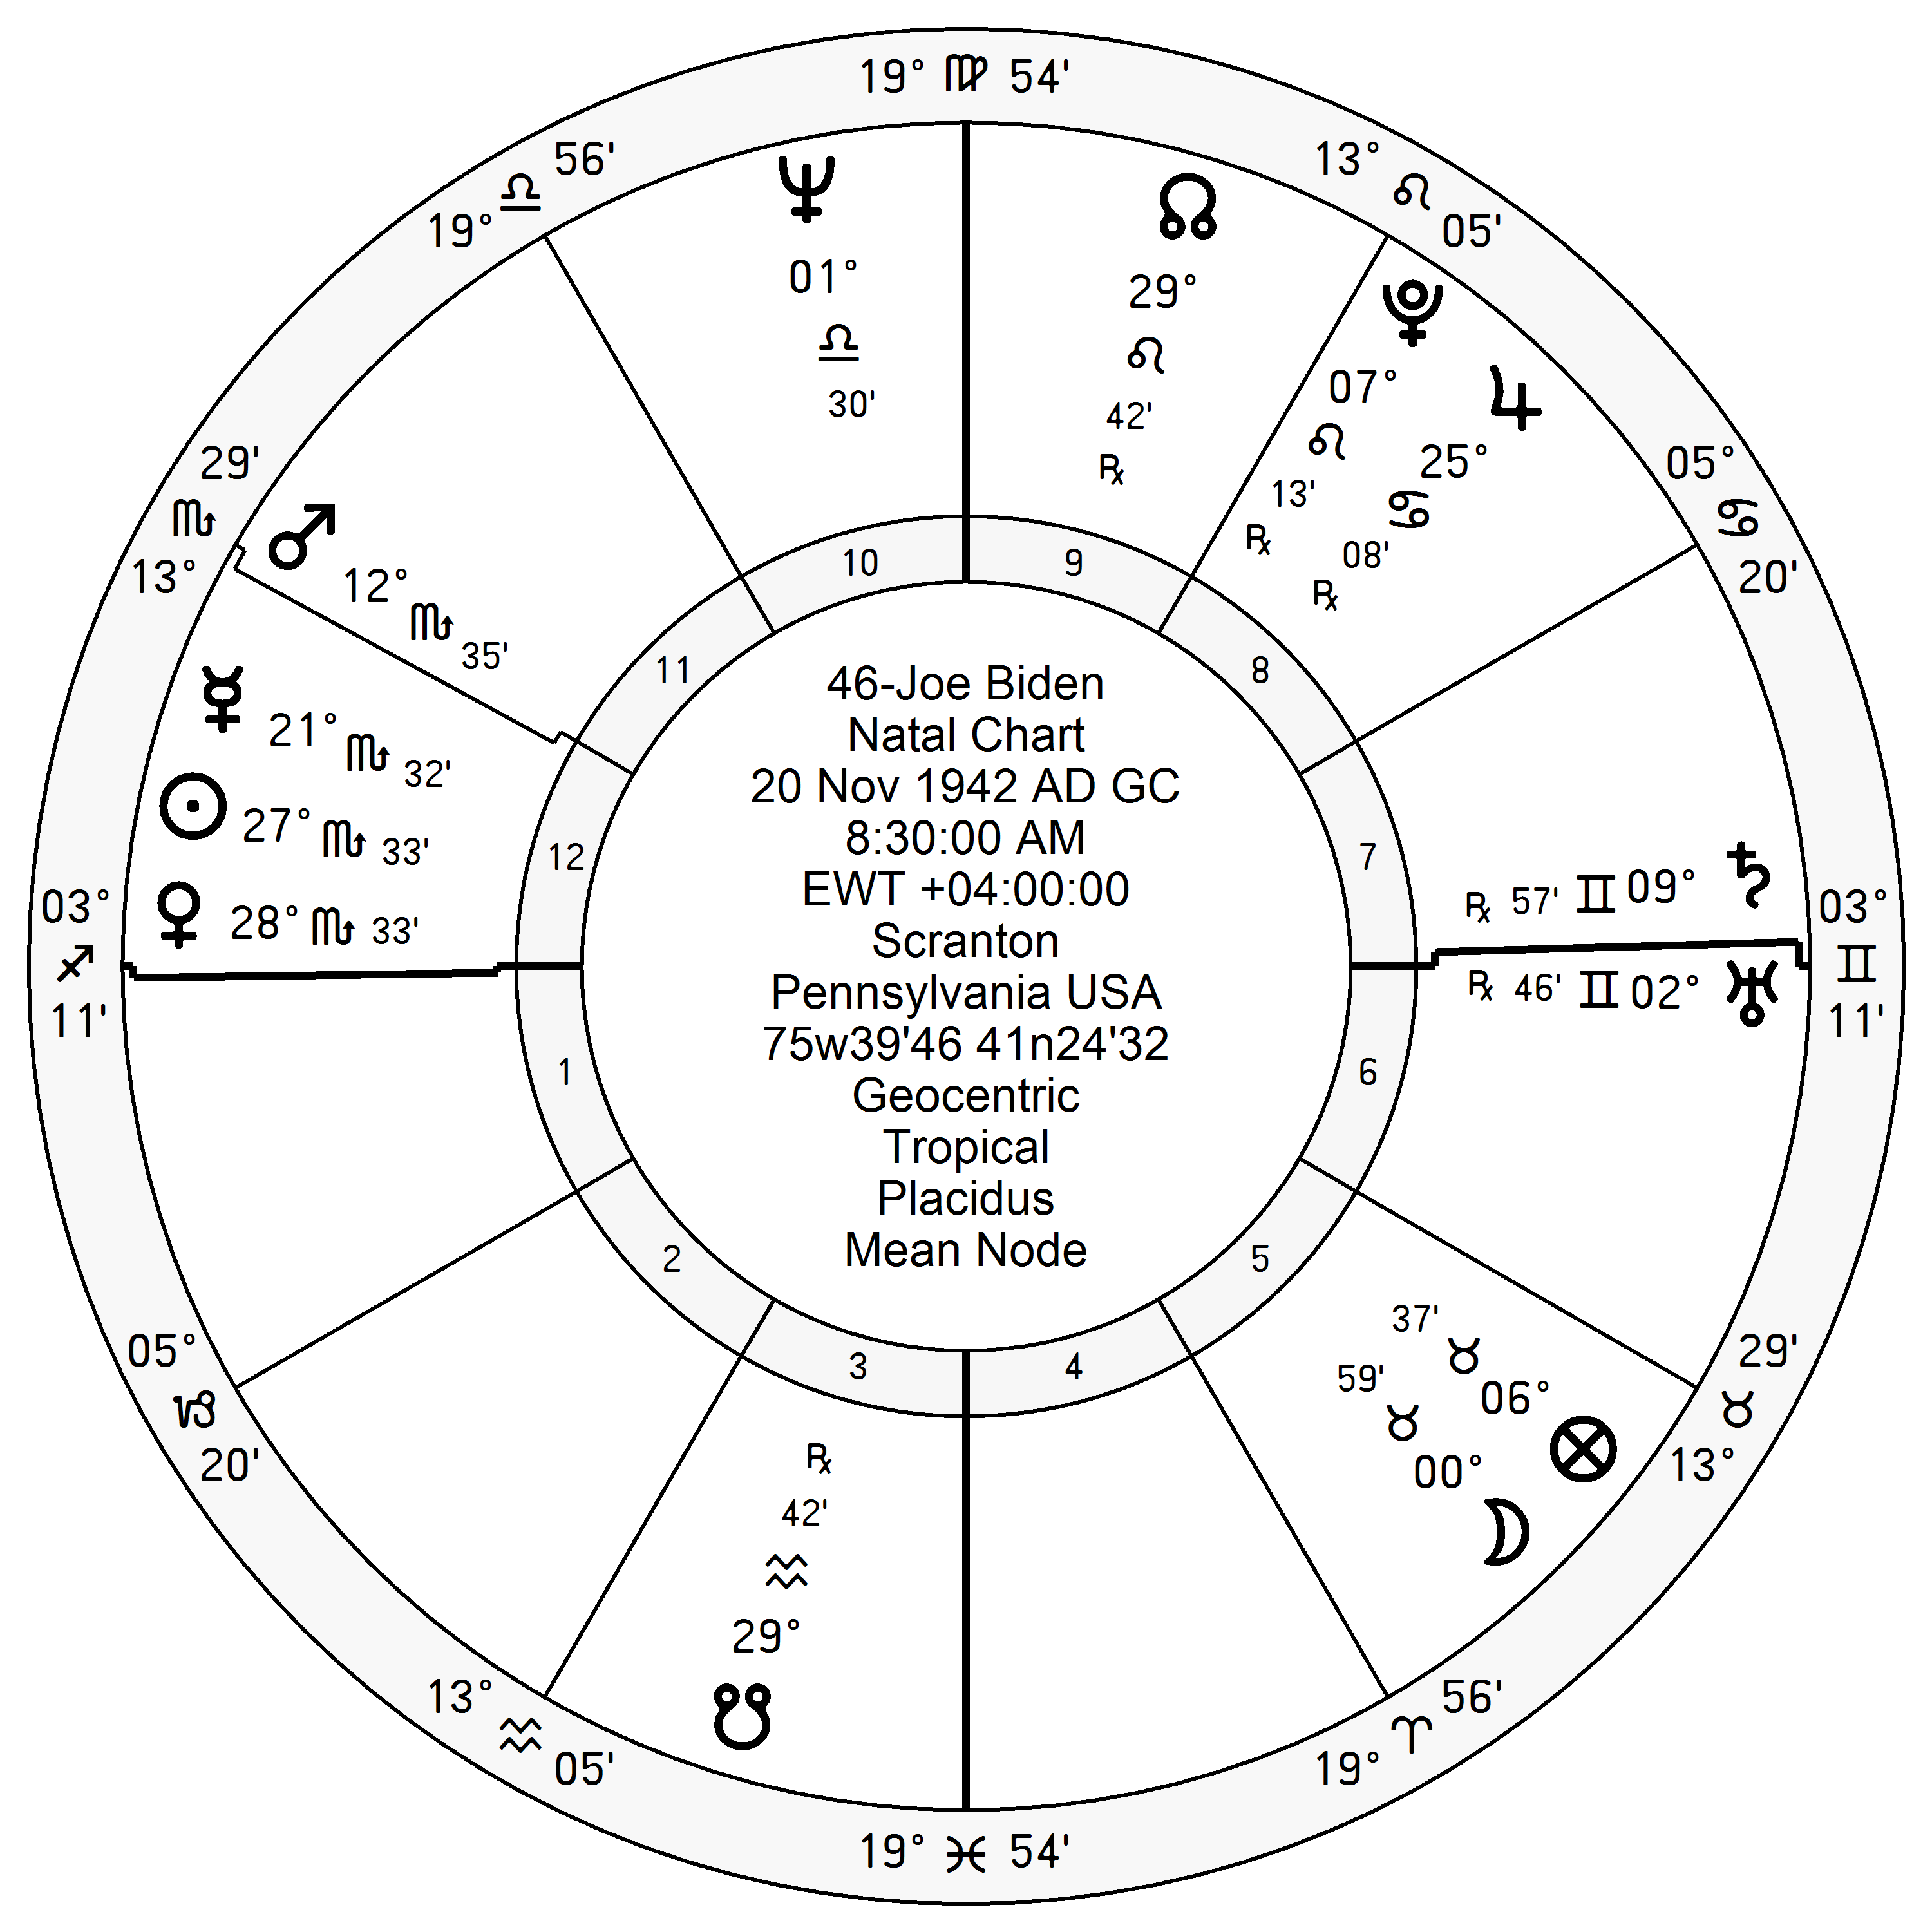
\includegraphics[width=0.9\textwidth]{charts/Biden.png}}
\fontsize{7pt}{8pt}\selectfont

\Mercury\, burnt \Sextile\, P1, \Sextile\, N10 \\
\Sun\, \Sextile\, P10; \Sextile\, N10

\column{0.48\textwidth}
\vspace{-1em}
{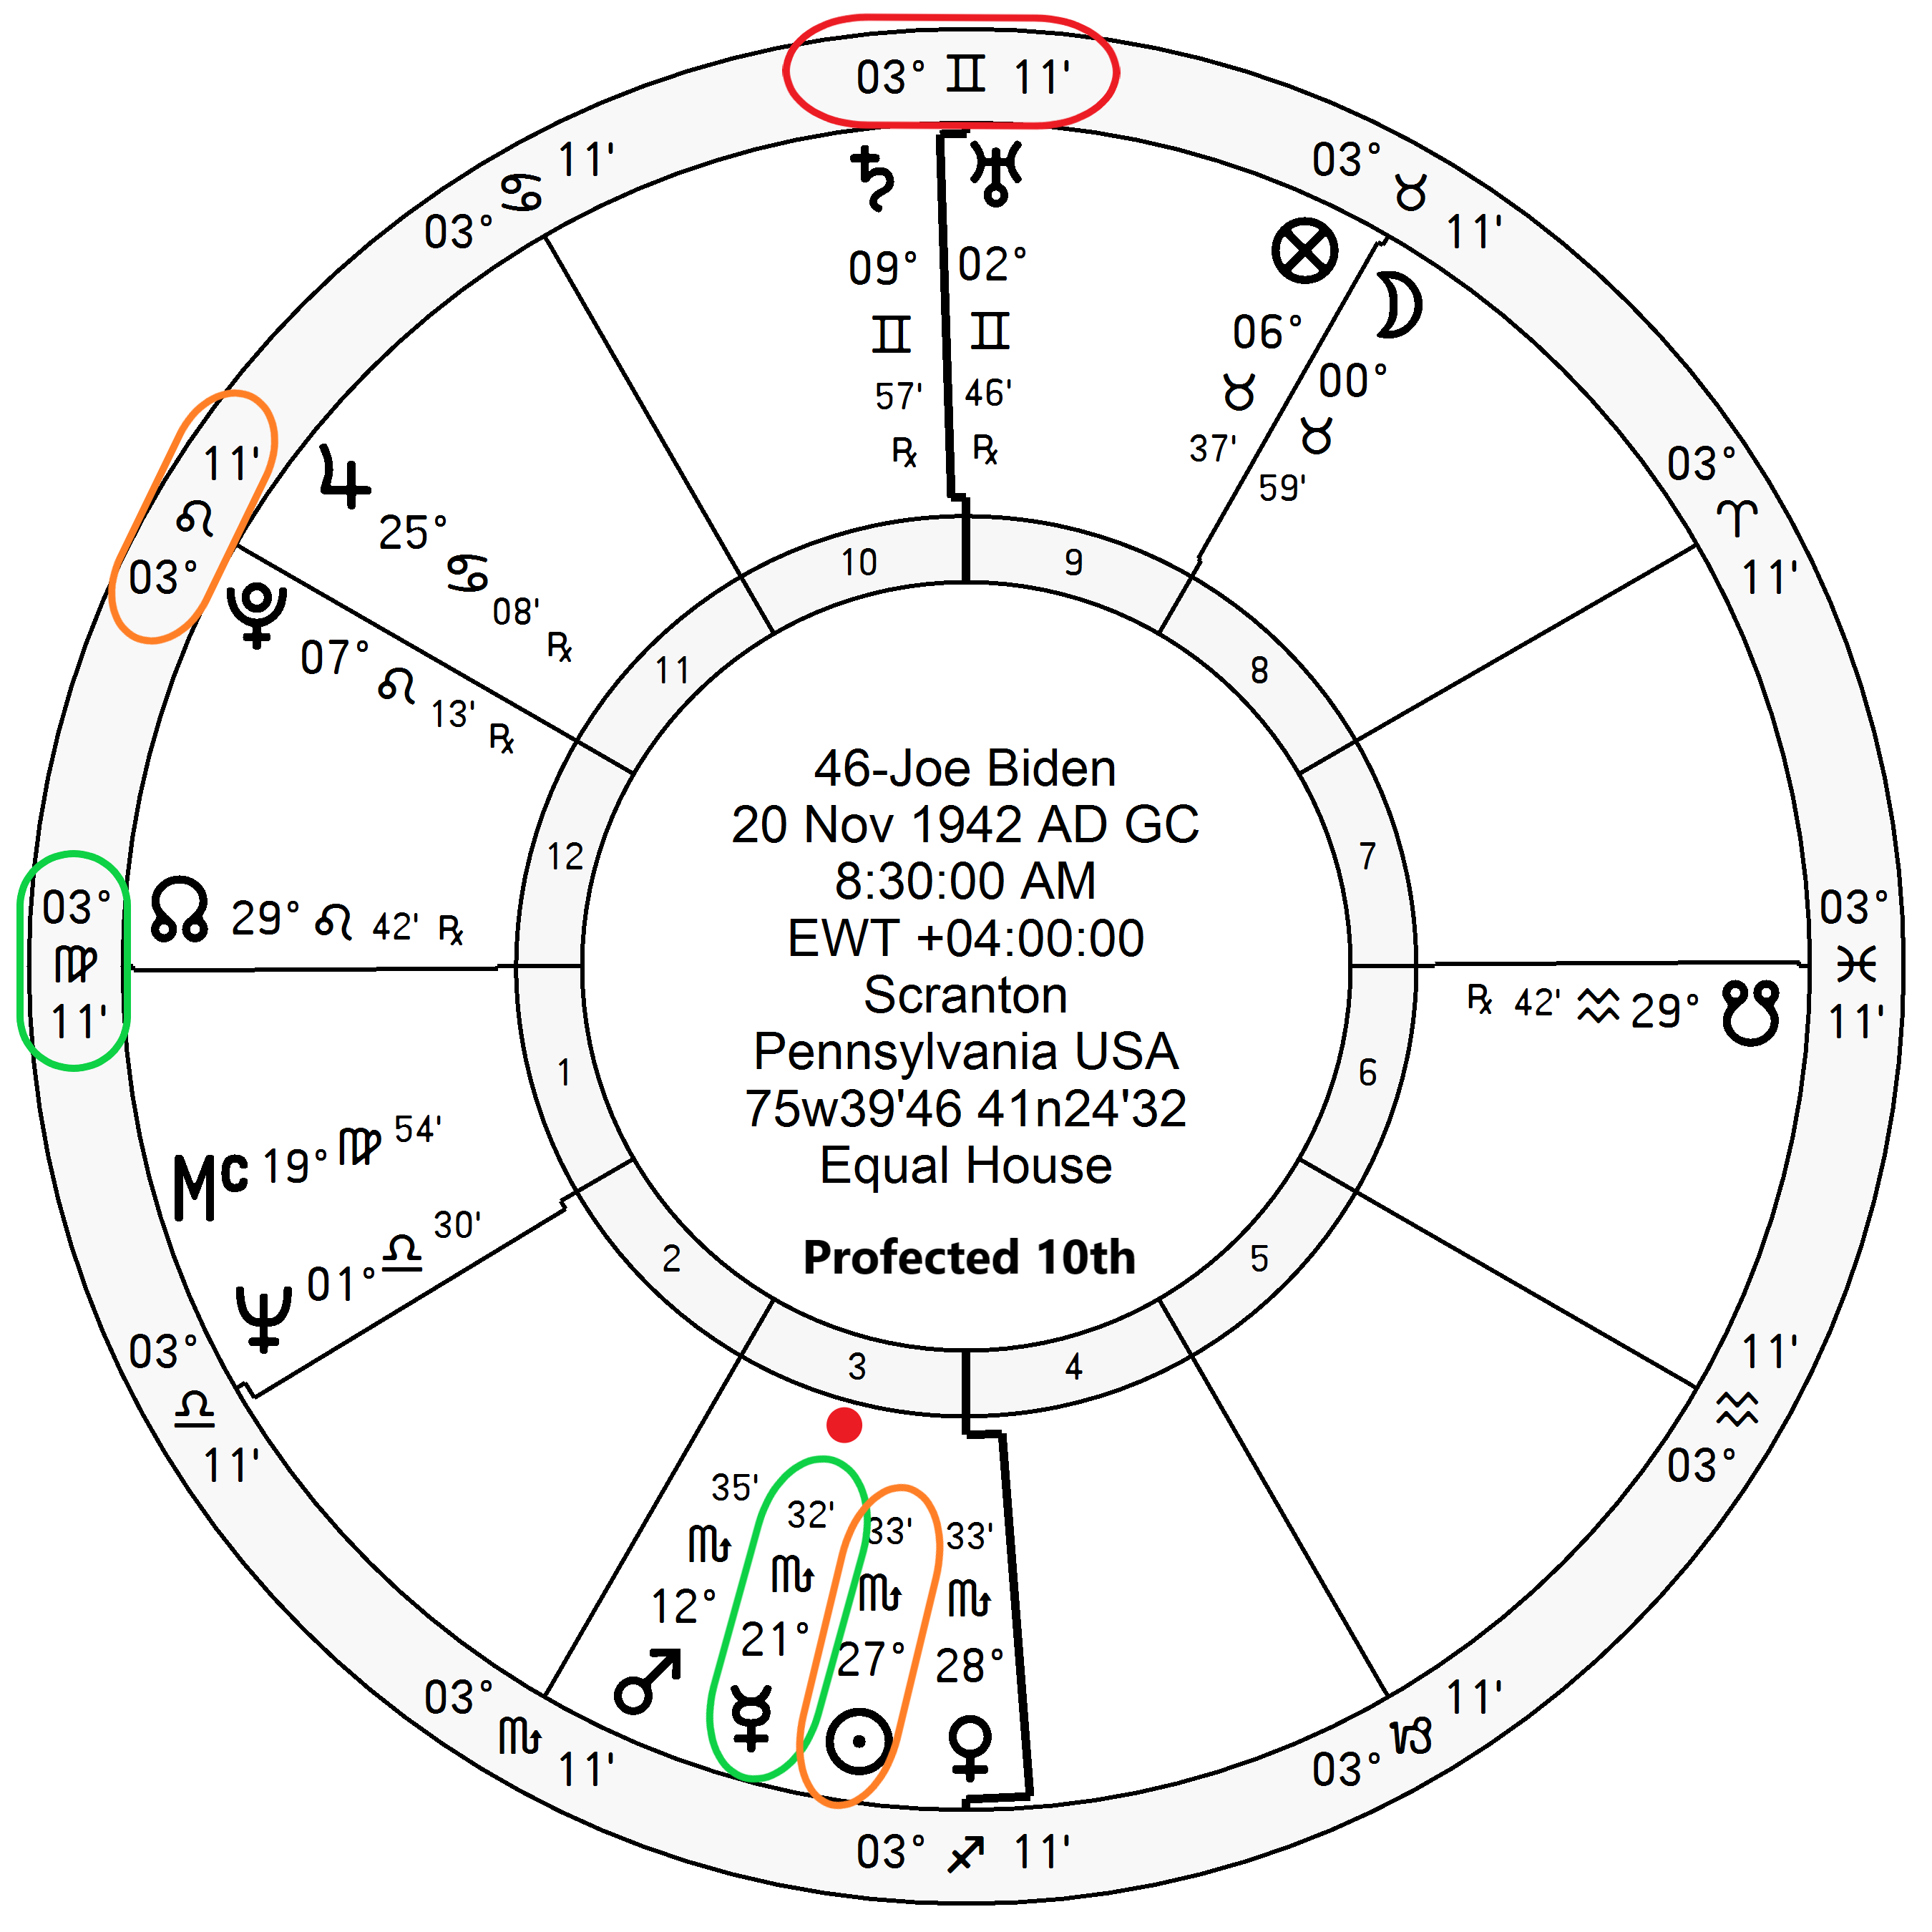
\includegraphics[width=0.9\textwidth]{charts/Biden-Prof-10th.png}}
\fontsize{8pt}{9pt}\selectfont

\textbf{\dgreen P1}=N10
	$\Rightarrow$ \Mercury\, (burnt) $\Rightarrow$ \textbf{\dgreen P3/N12}\\
\textbf{\red P10}=N7
	$\Rightarrow$ \Mercury\, (burnt) $\Rightarrow$ \textbf{\dgreen P3/N12}\\
PE=\textbf{\dgreen P12}/N9
	 $\Rightarrow$ \Sun\, $\Rightarrow$ \textbf{\dgreen P3/N12}

\end{columns}
\end{frame}

% ===================================================
\begin{frame}[t]{Election November 5, 2024: Donald Trump}
\small
\begin{columns}[T, onlytextwidth]
\column{0.48\textwidth}
\vspace{-1em}
{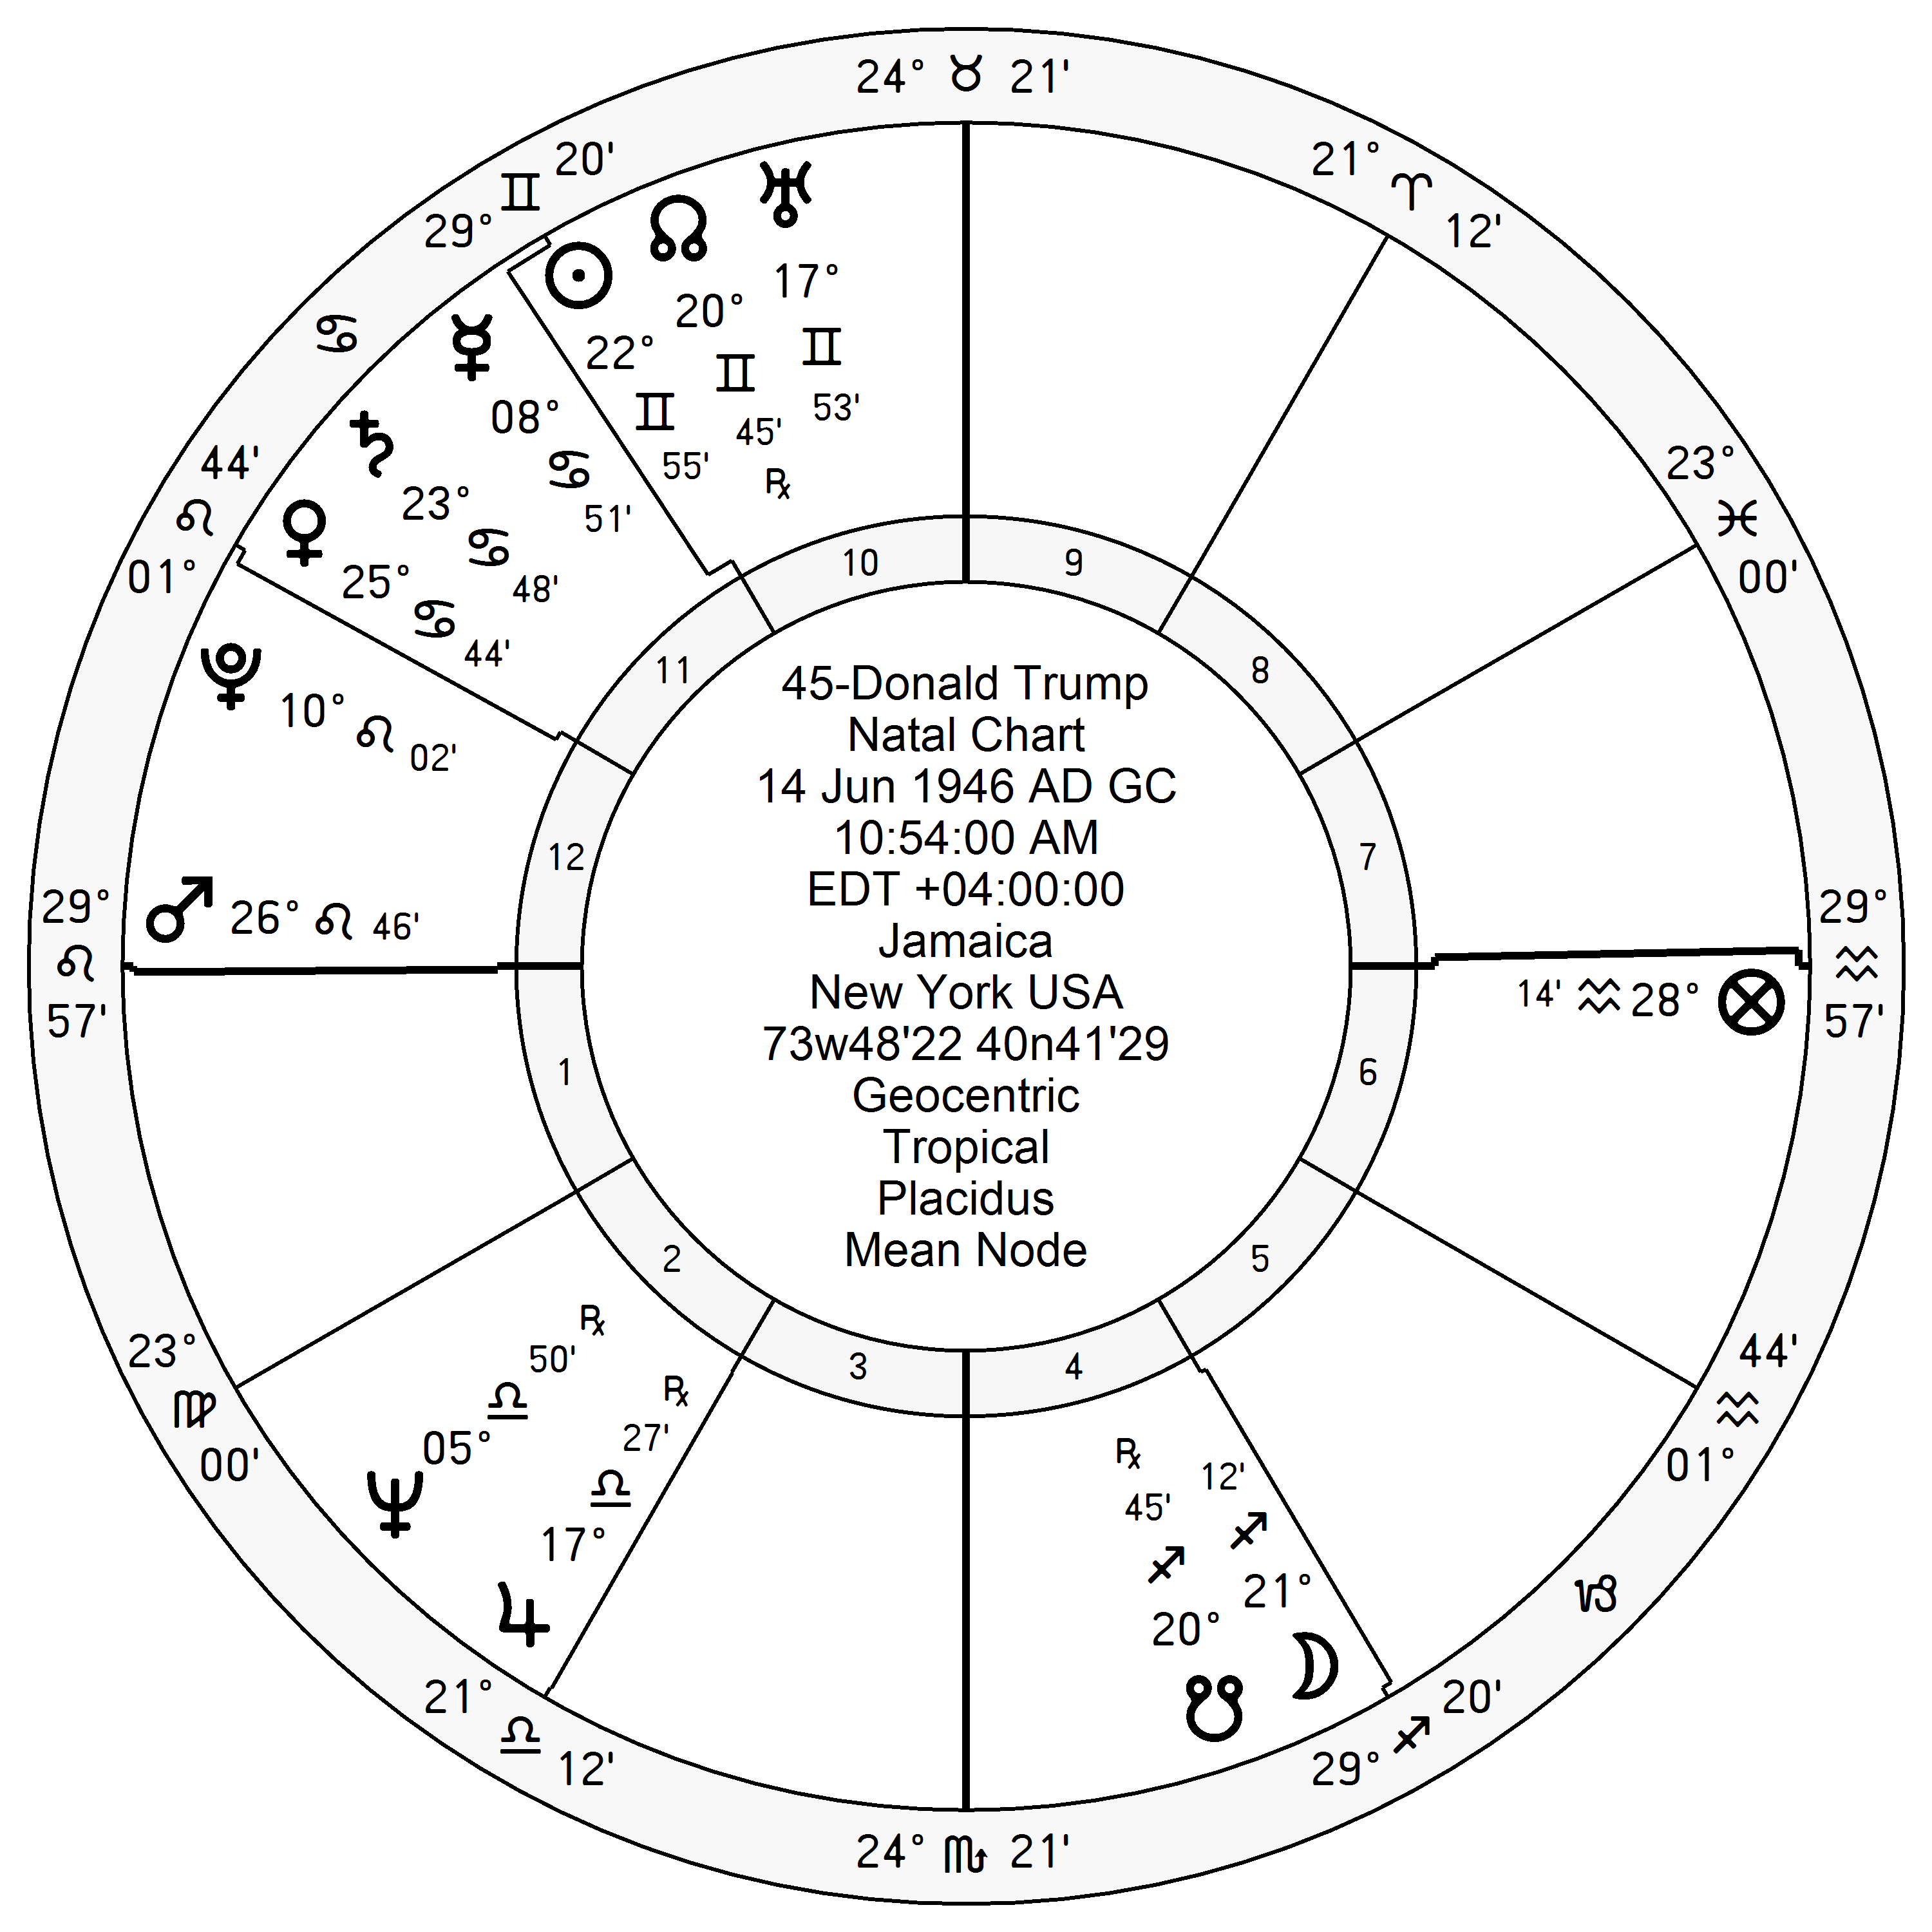
\includegraphics[width=0.9\textwidth]{charts/Trump.png}}
\fontsize{6pt}{7pt}\selectfont

\Saturn\, mit. \Quincunx\, (\Opposition) P10, \Trine\, P1, partile \Sextile\, to N2 \\
\Mars\, \Trine\, P10; \Square\, N10 \\
\Mercury\, \Trine\, P1, mit. \Quincunx\, (\Opposition) P10; \Sextile\, N1 \\
\vspace{0.5em}
Trump looks like the winner (assuming both are candidates on election day). The \SouthNode\, \Conjunction\, \Moon\, in P10 could cause problems, possibly GOP won't do well overall, weakening his control over Congress or the Senate, or both (\Moon\, rules P6, N11).

\column{0.48\textwidth}
\vspace{-1em}
{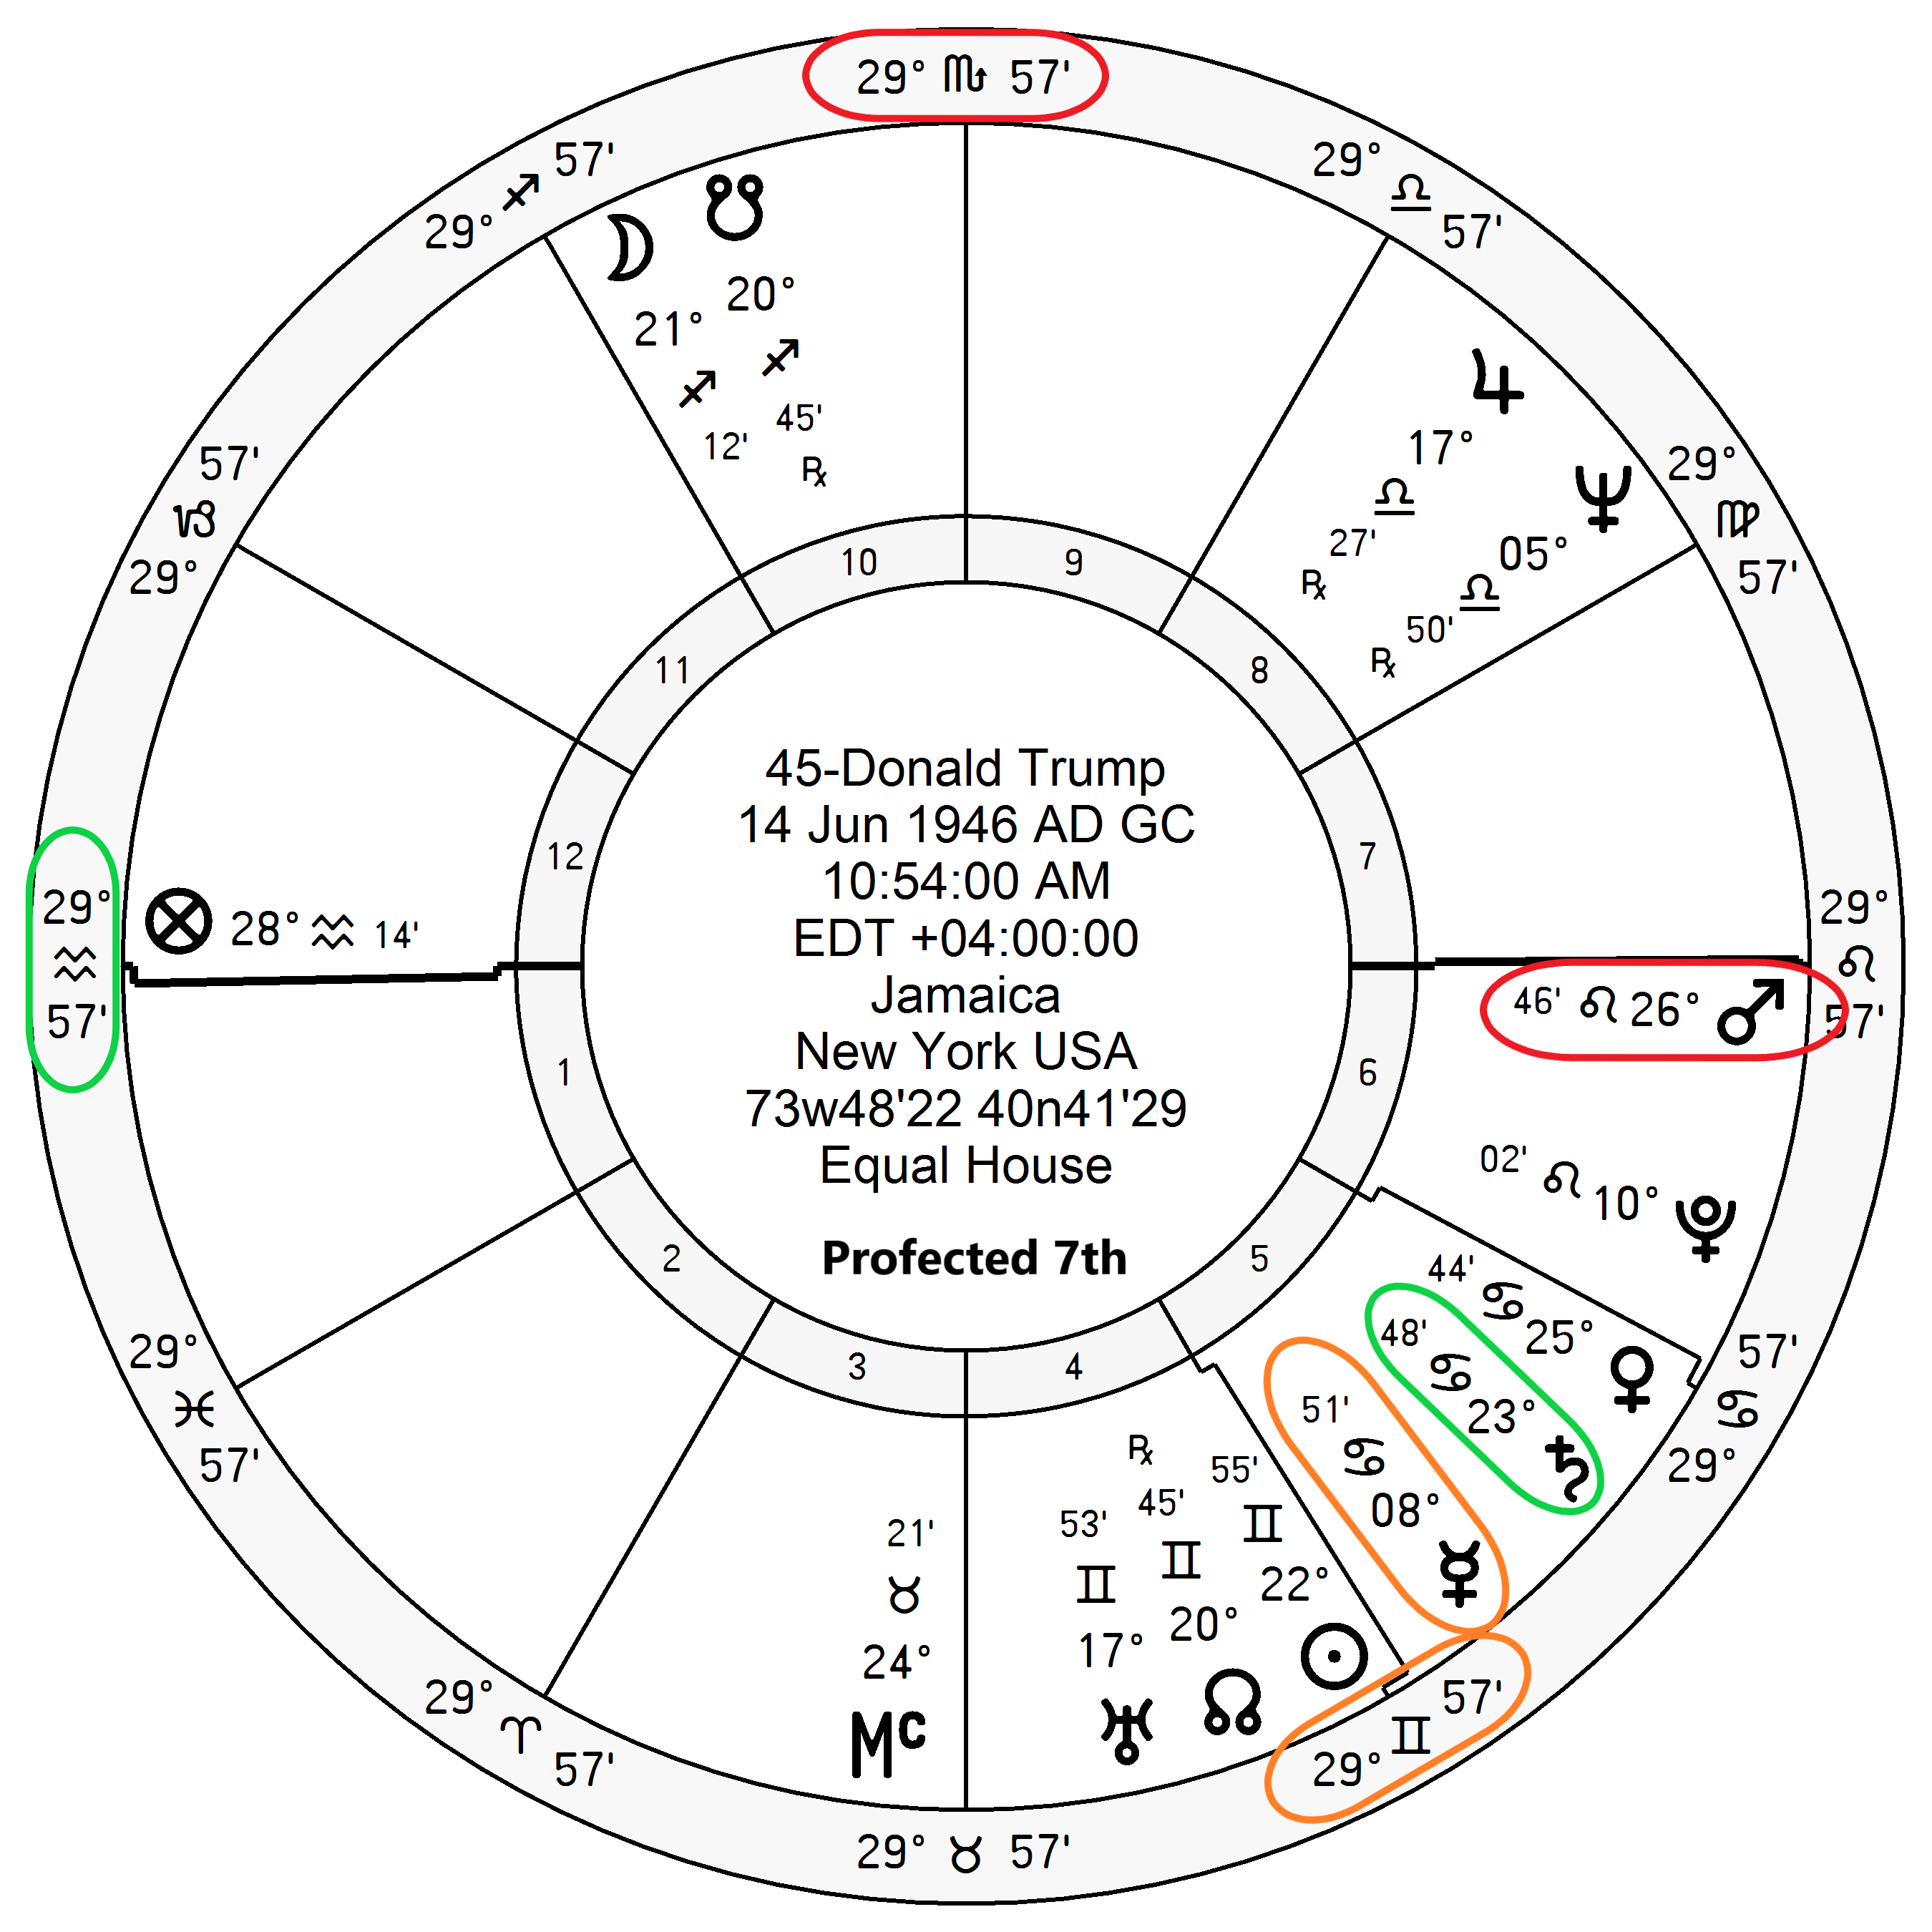
\includegraphics[width=0.9\textwidth]{charts/Trump-Prof-7th.png}}
\fontsize{8pt}{9pt}\selectfont
\textbf{\dgreen P1}=N7
	$\Rightarrow$ \Saturn\, $\Rightarrow$ \textbf{\dgreen P5/N11}\\
\textbf{\red P10}=N4
	$\Rightarrow$ \Mars\, $\Rightarrow$ P6/N12\\
PE=\textbf{\dgreen P5/N11}
	 $\Rightarrow$ \Mercury\, $\Rightarrow$ \textbf{\dgreen P5/N11}

\end{columns}
\end{frame}
% ===================================================
\begin{frame}[t]{Election November 5, 2024: Kamala Harris}
\small
\begin{columns}[T, onlytextwidth]
\column{0.48\textwidth}
\vspace{-1em}
{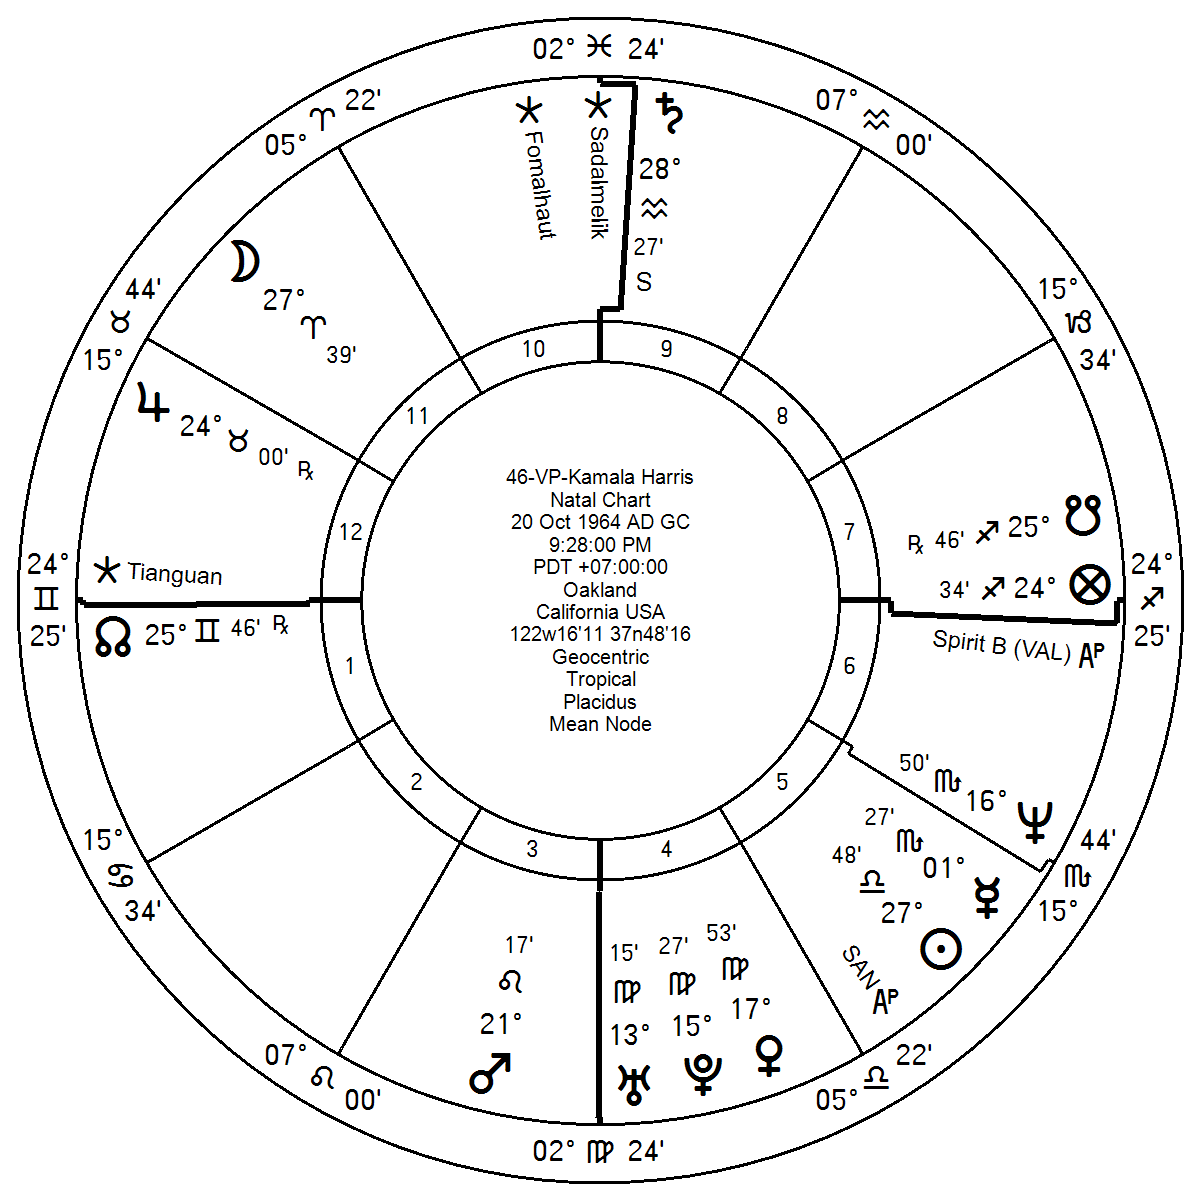
\includegraphics[width=0.9\textwidth]{charts/Harris.png}}
\fontsize{6pt}{7pt}\selectfont

\Mercury\, in P5 (elections) with \Sun\, (out of sign \Conjunction) with both in out of sign \Opposition\, to \Moon\, (changed conditions bring opposition?) \Trine\, MC \\
\Jupiter\, \Conjunction\, 12th (enemies) \Sextile\, 10th \\
\vspace{0.5em}
Possible the administration will put her in place as the candidate; the \NorthNode\, on the Asc could indicate a change in her status (MC is at the nodal bending) but it may not go well for her person (Fortune with \SouthNode). Chart does not look strong enough to pull off a win.

\column{0.48\textwidth}
\vspace{-1em}
{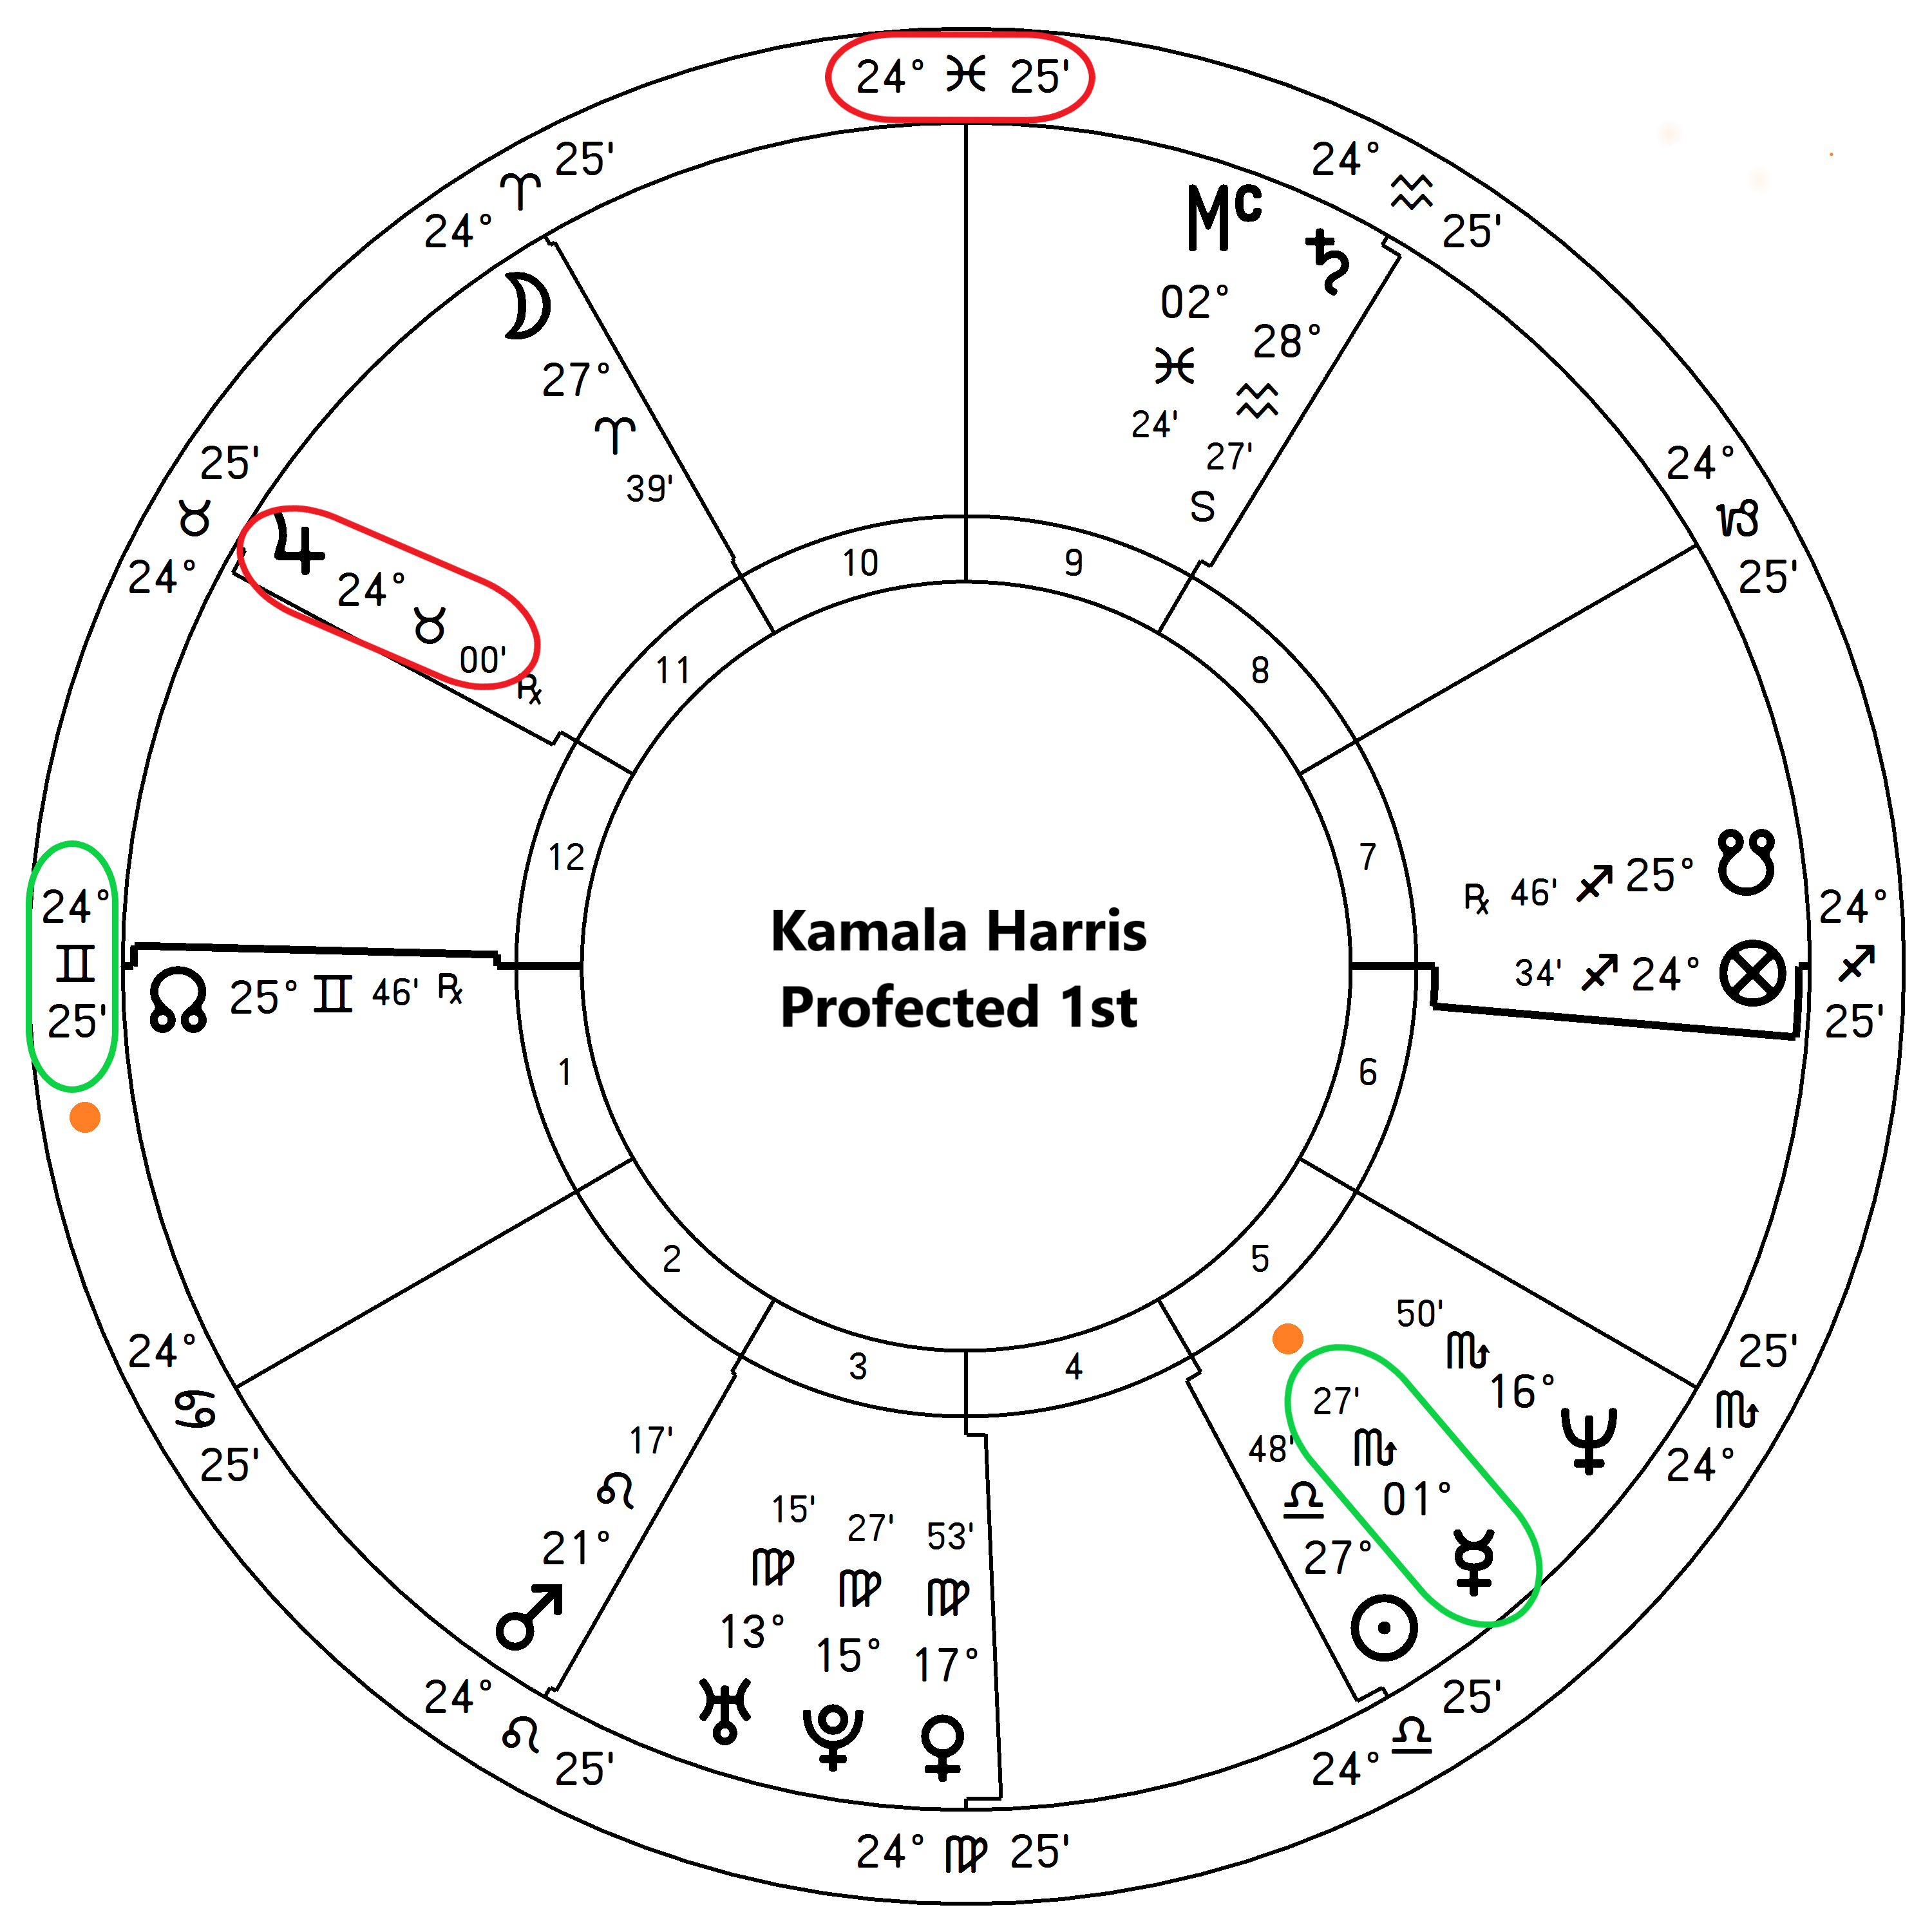
\includegraphics[width=0.9\textwidth]{charts/Harris-Prof-1st.png}}
\fontsize{8pt}{9pt}\selectfont
\textbf{\dgreen P1=N1}
	$\Rightarrow$ \Mercury\, $\Rightarrow$ \textbf{\dgreen P5/N5}\\
\textbf{\red P10}=N10
	$\Rightarrow$ \Jupiter\, $\Rightarrow$ P11/N12\\
PE=\textbf{\dgreen P1/N1}
	 $\Rightarrow$ \Mercury\, $\Rightarrow$ \textbf{\dgreen P5/N5}

\end{columns}
\end{frame}

